% 原书第295页；来源：用户补充截图 source-supplements/volume-2-p295.png。
唯一点列 $A=A_0,A_1,\ldots,A_l=B$，使得对 $0\leq i\leq l-1$，$A_i,A_{i+1}$ 相邻，且对 $1\leq i\leq l-1$，有 $A_{i-1}\ne A_{i+1}$。记 $l=l(A,B)$，称为 $A,B$ 之间的长度（length）。

(ii) 若 $A,B,A',B'\in\mathcal T^0$ 满足 $l(A,B)=l(A',B')$，且 $A,A'$ 属于同一陪集空间 $V_1\backslash G_{\mathfrak p}^+$ 或 $V_2\backslash G_{\mathfrak p}^+$，则存在 $g\in G_{\mathfrak p}^+$，使 $A'=A^g$、$B'=B^g$。
\end{originaltheorem}

特别地，$\mathcal T^0$ 为无限集，因此 $(G_{\mathfrak p}^+:V_0)=\infty$。此外，由(ii)得到 $(V_0:\{1\})=\infty$，即 $[L:K_0]=\infty$。这特别蕴含 $K_1\cap K_2=k_c$。由(i)直接得到：

\begin{originaltheorem}{推论 2.3.2（Corollary 2.3.2）}
$G_{\mathfrak p}^+$ 是 $V_1,V_2$ 关于公共子群 $V_0$ 的融合自由积。
\end{originaltheorem}

\paragraph*{2.4.}
$\mathcal T$ 的图形如下（$q=2$）：
\begin{center}
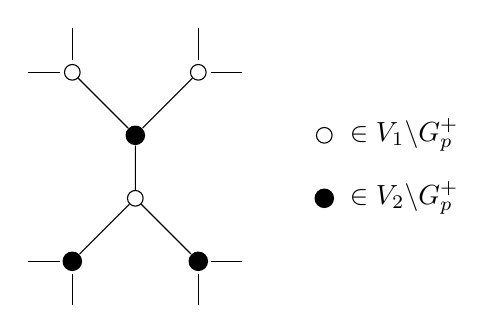
\begin{tikzpicture}[scale=.8]
 \node[circle,draw,inner sep=2pt] (a) at (-1,1.5) {};
 \node[circle,draw,inner sep=2pt] (b) at (1,1.5) {};
 \node[circle,fill=black,inner sep=2.5pt] (c) at (0,.5) {};
 \node[circle,draw,inner sep=2pt] (d) at (0,-.5) {};
 \node[circle,fill=black,inner sep=2.5pt] (e) at (-1,-1.5) {};
 \node[circle,fill=black,inner sep=2.5pt] (f) at (1,-1.5) {};
 \draw (a)--(c)--(b) (c)--(d)--(e) (d)--(f);
 \draw (-1,1.7)--(-1,2.2) (-1.2,1.5)--(-1.7,1.5)
       (1,1.7)--(1,2.2) (1.2,1.5)--(1.7,1.5)
       (-1,-1.7)--(-1,-2.2) (-1.2,-1.5)--(-1.7,-1.5)
       (1,-1.7)--(1,-2.2) (1.2,-1.5)--(1.7,-1.5);
 \node[circle,draw,inner sep=2pt] at (3,.5) {};
 \node[anchor=west] at (3.25,.5) {$\in V_1\backslash G_{\mathfrak p}^+$};
 \node[circle,fill=black,inner sep=2.5pt] at (3,-.5) {};
 \node[anchor=west] at (3.25,-.5) {$\in V_2\backslash G_{\mathfrak p}^+$};
\end{tikzpicture}\qquad(2.4.1)
\end{center}
这正是与群 $\operatorname{PGL}_2(k)$ 对应的树。

\paragraph*{注 2.4.2.}
群 $G_{\mathfrak p}^+$ 与 $\operatorname{PGL}_2^+(k)$ 忠实作用于“同一个”图 $\mathcal T$，而且顶点轨道相同，分别为空心顶点和实心顶点。已有例子表明，若不对 $\mathcal X$ 施加非分歧等条件，$G_{\mathfrak p}^+$ 可以严格大于 $\operatorname{PGL}_2^+(k)$。

\paragraph*{2.5.}
定理2.3.1的证明只基于下述事实：“存在 $K_1$ 的离散赋值 $v_1$、$K_2$ 的离散赋值 $v_2$，及 $K_0$ 的离散赋值 $w_1,w_2$，满足：(a) 对每个 $i=1,2$，$w_1,w_2$ 为 $v_i$ 到 $K_0$ 的全部不同延拓；(b) 对每个 $i=1,2$，$K_i$ 在 $K_0$ 中关于 $w_i$ 进拓扑稠密。”局部环 $\mathcal O_{X_i,X_{is}}$、$\mathcal O_{X_0,\Pi}$、$\mathcal O_{X_0,{}^t\Pi}$ 定义了具有这些性质的赋值 $v_i,w_1,w_2$。

\paragraph*{2.6.}
令 $\overline k\cap L$ 为 $k$ 在 $L$ 中的代数闭包。$G_{\mathfrak p}^+$ 作用于 $\overline k\cap L$，且不动域为 $k_c$。因此 $(\overline k\cap L)/k_c$ 为 Galois 扩张。若用 $\overline{G_{\mathfrak p}^+}$ 表示 $G_{\mathfrak p}^+$ 在 $\overline k\cap L$ 上作用的核，则有典范同构
\[
 \Aut((\overline k\cap L)/k_c)
 \simeq G_{\mathfrak p}^+/\overline{G_{\mathfrak p}^+}.
\]
关于 $\overline k\cap L$ 的“大小”，以下断言已经足够。

\begin{originaltheorem}{命题 2.6.1（Proposition 2.6.1）}
对任意 $g,g'\in G_{\mathfrak p}^+$ 及 $1\leq i,j\leq2$，$k_c$ 在 $K_i^g\cdot K_j^{g'}$ 中代数闭；换言之，
\[
 G_{\mathfrak p}^+
 =\bigl[(g^{-1}V_ig)\cap((g')^{-1}V_jg')\bigr]
 \cdot\overline{G_{\mathfrak p}^+}.
\]
\end{originaltheorem}
利用上述赋值 $v_i,w_i$ 的基本性质，容易证明此命题。

\paragraph*{2.7.}
当 $\mathcal X$ 对称时，等式 $X_2=X_1$ 定义同构 $K_1\xrightarrow{\sim}K_2$；由于 ${}^tT=T$，此同构唯一扩张为 $K_0$ 的一个对合，记为 $\iota$。在情形2中，$\iota$ 在 $k_2/k$ 上诱导一个对合。由 $L$ 的定义，$\iota$ 可延拓为 $L$ 的自同构，仍
